\section{Introduction}

The Helmholtz equation has the general form
\begin{equation}
    \label{eq:general}
    -\nabla^2{u(\underline{x})} - k^2 u(\underline{x}) = f(\underline{x}), \qquad \underline{x} \in \Omega
\end{equation}
and represents a time-independent form of the wave equation after applying the technique of separation of variables.
This equation often arises in various physical problems including the study of electromagnetic radiation, seismology,
and acoustics.\\
** elaborate on the importance of the equation **\\
** literature review on the numerical schemes **\\

In this study, we will consider the 1-dimensional Helmholtz equation with impedance boundary conditions in the domain $\Omega=[a, b]$
\begin{equation}
    \label{eq:main}
    \begin{aligned}
        -u''(x) - k^2 u(x) = f(x)\\
        -u'(a) - \imath k^2 u(a) = g_a \in \mathbb{C}\\
        +u'(b) - \imath k^2 u(b) = g_b \in \mathbb{C}
    \end{aligned}
\end{equation}
where $k$ is often called the frequency of the equation, as larger values of this parameter result in more oscillating solutions.
** why impedance boundary conditions? **
We will mainly consider \autoref{eq:main} in the domain $[-1,\:+1]$.

With the recent improvements in knowledge and practical aspects of machine learning techniques, and more specifically,
deep learning and neural networks, these methods are being successfully implemented in domains and applications such as
computer vision, recommender systems, generative models, etc., where they can benefit from the abundance of data and
learn the features that best represent the problem.
However, in the context of analyzing complex physical, biological, or engineering systems, these methods are facing
the challenge of high cost of data acquisition, which forces us to find a way to make decisions in an semi-supervised
fashion while retaining the robustness and convergence of the methods.

Recent studies in the literature have introduced deep learning frameworks for solving nonlinear partial differential
euqations (PDEs) that have achieved this goal.

Raissi \textit{et. al.} \cite{RAISSI2019686} have introduced the physics-informed neural networks (PINNs) scheme,
which uses the prior knowledge that usually stems from the physics of the system in a structured way as a regularization
method to narrow the range of the admissible solutions. They consider the general form of a nonlinear PDE as
\begin{equation}
    u_t + N[u; \lambda] = 0, x \in \Omega, t \in [0, T]
\end{equation}
where $u(t, x)$ denotes the unknown solution, $N[.; \lambda]$ is a nonlinear operator parameterized by $\lambda$,
and $\Omega$ is a subset which defines the domain of the system. With $f(t, x)$ as the left-hand-side of this equation,
the method consists of defining two neural networks for $u(t, x)$ and $f(t, x)$ with shared parameters,
and optimizing these parameters based on a suitable loss function that takes into account the initial condition,
boundary conditions, and satisfaction of the equation in quadrature points of the domain. They have shown that their
method performs well even with small data for several nonlinear PDEs by comparing their results with the exact solution
of those equations.\\

Kharazmi \textit{et. al.} \cite{kharazmi2019variational} have taken the next step by developing a Petrov-Galerkin
version of the PINNs by selecting the trial space to be the space of the neural networks and the test space to be the
space of trigonometric functions or Legendre polynomials. They introduce the variational physics-informed neural networks
(VPINNs) by incorporating the variational residual of the PDE in the loss function of the network. They show that by
integrating by parts the integrand part of the variational form, they can reduce the training time of the VPINNs and
increase their accuracy compared to PINNs. They obtain the explicit form of the variational residual for shallow neural
networks with one hidden layer, and suggest that numerical integration techniques should be employed for deep neural
networks.\\

The goal of this study is to implement the VPINNs scheme introduced in \cite{kharazmi2019variational} for solving
\autoref{eq:main} and to explore the behavior of these networks with different structures, activation functions, etc.
and for different parameters of the equation.
For this purpose, we will present the variational formulation of \autoref{eq:main} in \autoref{sec:frameworks}.
Then, we will proceed with presenting the frameworks of a finite elements scheme and a VPINN scheme in \autoref{sec:femframework}
and \autoref{sec:vpinnsframework}, respectively. In \autoref{sec:results}, we will show the results of the implemented frameworks with various
parameters and conditions, which then will be discussed in \autoref{sec:discussion}. Section \ref{sec:conclusion} summerizes our conclusions and
provides some suggestions for future works.

\section{Frameworks and methods}\label{sec:frameworks}
** empty **

\subsection{Variational formulation of the Helmholtz problem}\label{sec:variational}

We take the 1-D version of the Helmholtz equation as expressed in \autoref{eq:main}, and test this equation by a
arbitrary smooth test function $v \in {H_{0}^{1} }_{(\Omega)}$ with compact support in the domain, to get
\begin{equation}
    \label{eq:tested}
    \int_{\Omega}{{(-u'' - k^2u)}v} = \int_{\Omega}{fv} \qquad \forall v \in {H_{0}^{1} }_{(\Omega)}.
\end{equation}

Integration by parts gives $\int_{a}^{b}{u''v} = [u'v]_{a}^{b} - \int_{a}^{b}{u'v'}$ which could be
replaced into \autoref{eq:tested} to eliminate the second derivative from the equation. Doing this, and by setting
$u'(a)v(a) = (-g_a-\imath ku(a))v(a)$ and $u'(b)v(b) = (g_b+\imath ku(b))v(b)$, we get the variational formulation
of the Helmholtz impedance problem, which is to find $u \in {H^{1} }_{(\Omega)}$ such that $a(u,\:v) = b(v)$ for all
$v \in {H_{0}^{1} }_{(\Omega)}$, where $a(u,\:v)$ and $b(v)$ are defind as

\begin{equation}
    \label{eq:varlhs}
    a(u,\:v) = \int_{a}^{b}{u'v'} - k^2 \int_{a}^{b}{uv} - \imath k (u(a)v(a) + u(b)v(b))
\end{equation}
\begin{equation}
    \label{eq:varrhs}
    b(v) = \int_{a}^{b}{fv} + g_a v(a) + g_b v(b)
\end{equation}

\subsection{Framework of the finite elements scheme}\label{sec:femframework}
We descritize the domain $\Omega=[a,\:b]$ by defining $N+1$ basis functions as
\begin{equation}
    \label{eq:fembasisfuncs}
    \varphi_j(x) = \left\{\begin{matrix}
        1 - \frac{N}{2}|x - x_j|, \quad x_{j-1} < x < x_{j+1}
        \\
        0, \qquad \qquad otherwise.
        \end{matrix}\right.
\end{equation}
for $j = 0, \cdots, N+1$. The resulting basis functions with $N=9$ are illustrated in \autoref{fig:fembases}. Let
$V_N = span(\varphi_j)_{j=0, \cdots, N+1} \subset H^{1}$ be a finite-dimensional subset of $H^{1}$. We search for
solutions in this subspace, and modify the variational version of the Helmholtz impedance problem as finding
$u_N \in V_N$ such that $a(u_N,\:v_N) = b(v_N)$ for all $v_N \in V_N$, where $a(u,\:v)$ and $b(v)$ are defind in Equations
\ref{eq:varlhs} and \ref{eq:varrhs}, respectively. We can easily see that it is actually sufficient to ensure that the aforementioned
equation is satisfied for all the basis functions $\varphi_i,\:i=0, \cdots, N+1$:
\begin{equation}
    \label{eq:femvar}
    a(u_N,\:\varphi_i) = b(\varphi_i)
\end{equation}
Let $u_N \in V_N$ be a linear combination of the basis of $V_N$, $u_N(x) = \sum_{j=0}^{N}{c_j\varphi_j}$. By plugging
$u_N$ into \autoref{eq:femvar}, we can verify that the stated problem could be expressed as a linear system of equations
$A\underline{c}=\underline{f}$, where
\begin{equation}
    \label{eq:femcoeffs}
    A = \begin{bmatrix}
        a(\varphi_0,\:\varphi_0) & a(\varphi_1,\:\varphi_0) & \cdots & a(\varphi_N,\:\varphi_0) \\
        a(\varphi_0,\:\varphi_1) & a(\varphi_1,\:\varphi_1) & \cdots & a(\varphi_N,\:\varphi_1) \\
        \vdots & \vdots & \ddots & \vdots \\
        a(\varphi_N,\:\varphi_N) & a(\varphi_0,\:\varphi_N) & \cdots & a(\varphi_N,\:\varphi_N)
        \end{bmatrix},
        \quad
        \underline{c} = \begin{bmatrix}
        c_0\\
        c_1\\
        \vdots\\
        c_N
        \end{bmatrix},
        \quad
        \underline{f} = \begin{bmatrix}
        b(\varphi_0)\\
        b(\varphi_1)\\
        \vdots\\
        b(\varphi_N)
        \end{bmatrix}.
\end{equation}
The solution of this system of equations could be calculated using methods such as Gauss-elimination. We don't need
any quadrature rule to calculate the integrals in $a(\varphi_j,\:\varphi_i)$ as these result in determined values depending
on $i$ and $j$.

\begin{figure}[h]
    \label{fig:fembases}
    \centering
    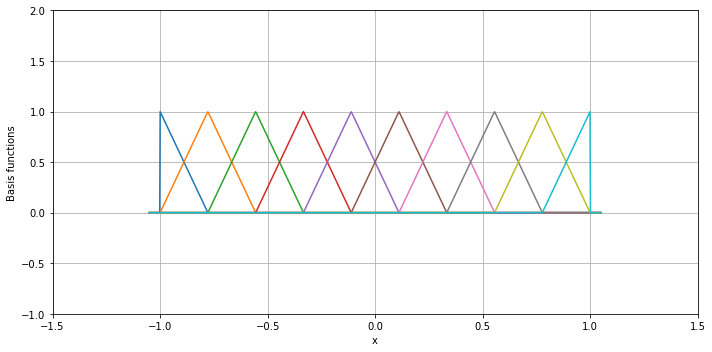
\includegraphics[width = 0.6\textwidth]{img/FEMBasisFunctions.png}
    \caption{The finite element basis functions over the domain $\Omega = [a,\:b]$ for $N=9$.}
\end{figure}

\subsection{Framework and structure of the VPINNs scheme}\label{sec:vpinnsframework}

\subsubsection{Multilayer perceptron}\label{sec:vpinnsmlp}
Let $NN$ be the space of a fully-connected multilayer perceptron (MLP) with 1 node at the input layers,
$N$ nodes on each of $D$ hidden layers, and 2 nodes at the output layer as depicted in \autoref{fig:vpinndeepmlp}.
The 2 dimensional output represents the real and the imaginary part of the solution
$u_N(x) = u_{N,\;1}(x) + \imath u_{N,\;2}(x)$. In case of shallow networks, it could be easily shown that this will
be the same as using complex model parameters.\\
For this generic structure of the MLP, each element of the the 2-dimensional solution could be expressed as
\begin{equation}
    \label{eq:vpinngeneric}
    u_{N,\;i} = c_0^i + \sum_{j=1}^{N}{c_j^i \sigma(h^{D} \circ h^{D-1} \circ \cdots \circ h^1(x))},
\end{equation}
where $\sigma (x)$ is a non-linear activation function, $h^1_i = \sigma(w^1_i x + b^1_i)$, and
$h^d_i = \sigma(\sum_{n=1}^{N}{w^d_{i, n} h^{d-1}_n} + b^d_i)$ for $d = 2, \cdots, D$.
**Put figures of MLP and shallow network with parameter names**
\begin{figure}[h]
    \centering
    \begin{subfigure}[b]{0.45\textwidth}
        \label{fig:vpinndeepmlp}
        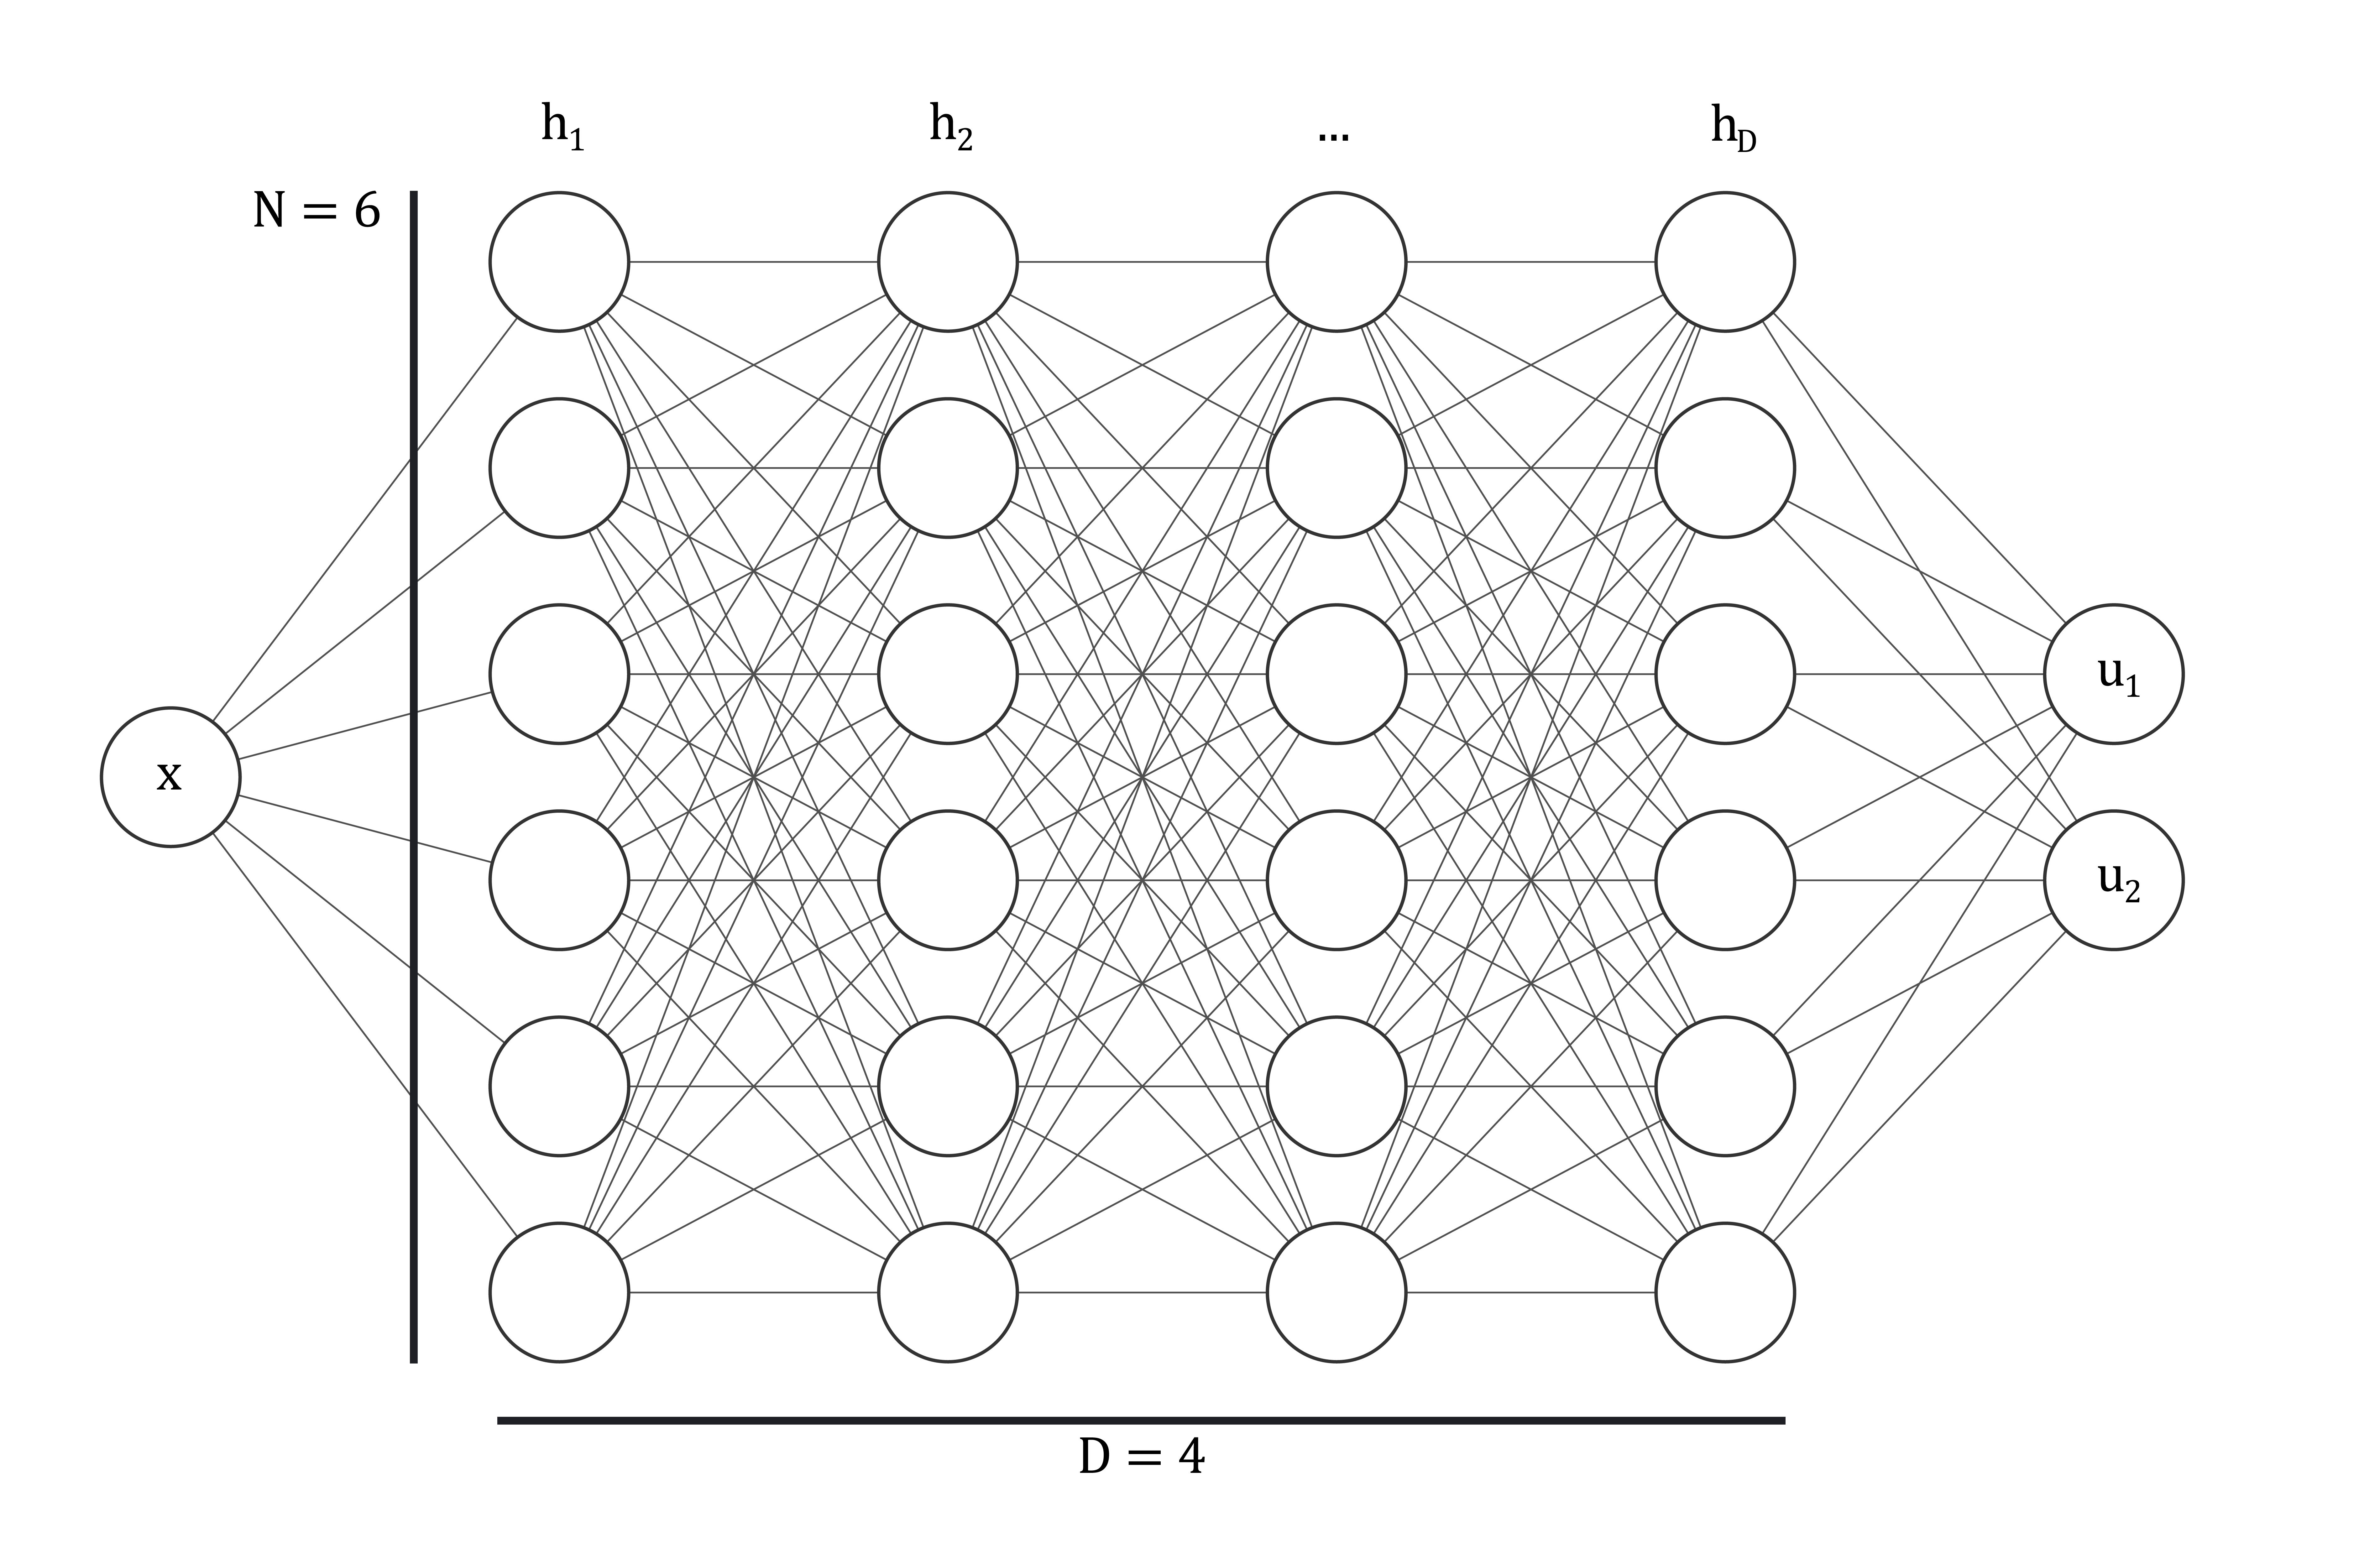
\includegraphics[width=\textwidth]{img/DeepMLP.png}
        \caption{Generic mulilayer perceptron with 4 hidden layer and $N=6$.}
    \end{subfigure}
    \hfill
    \begin{subfigure}[b]{0.45\textwidth}
        \label{fig:vpinnshallowmlp}
        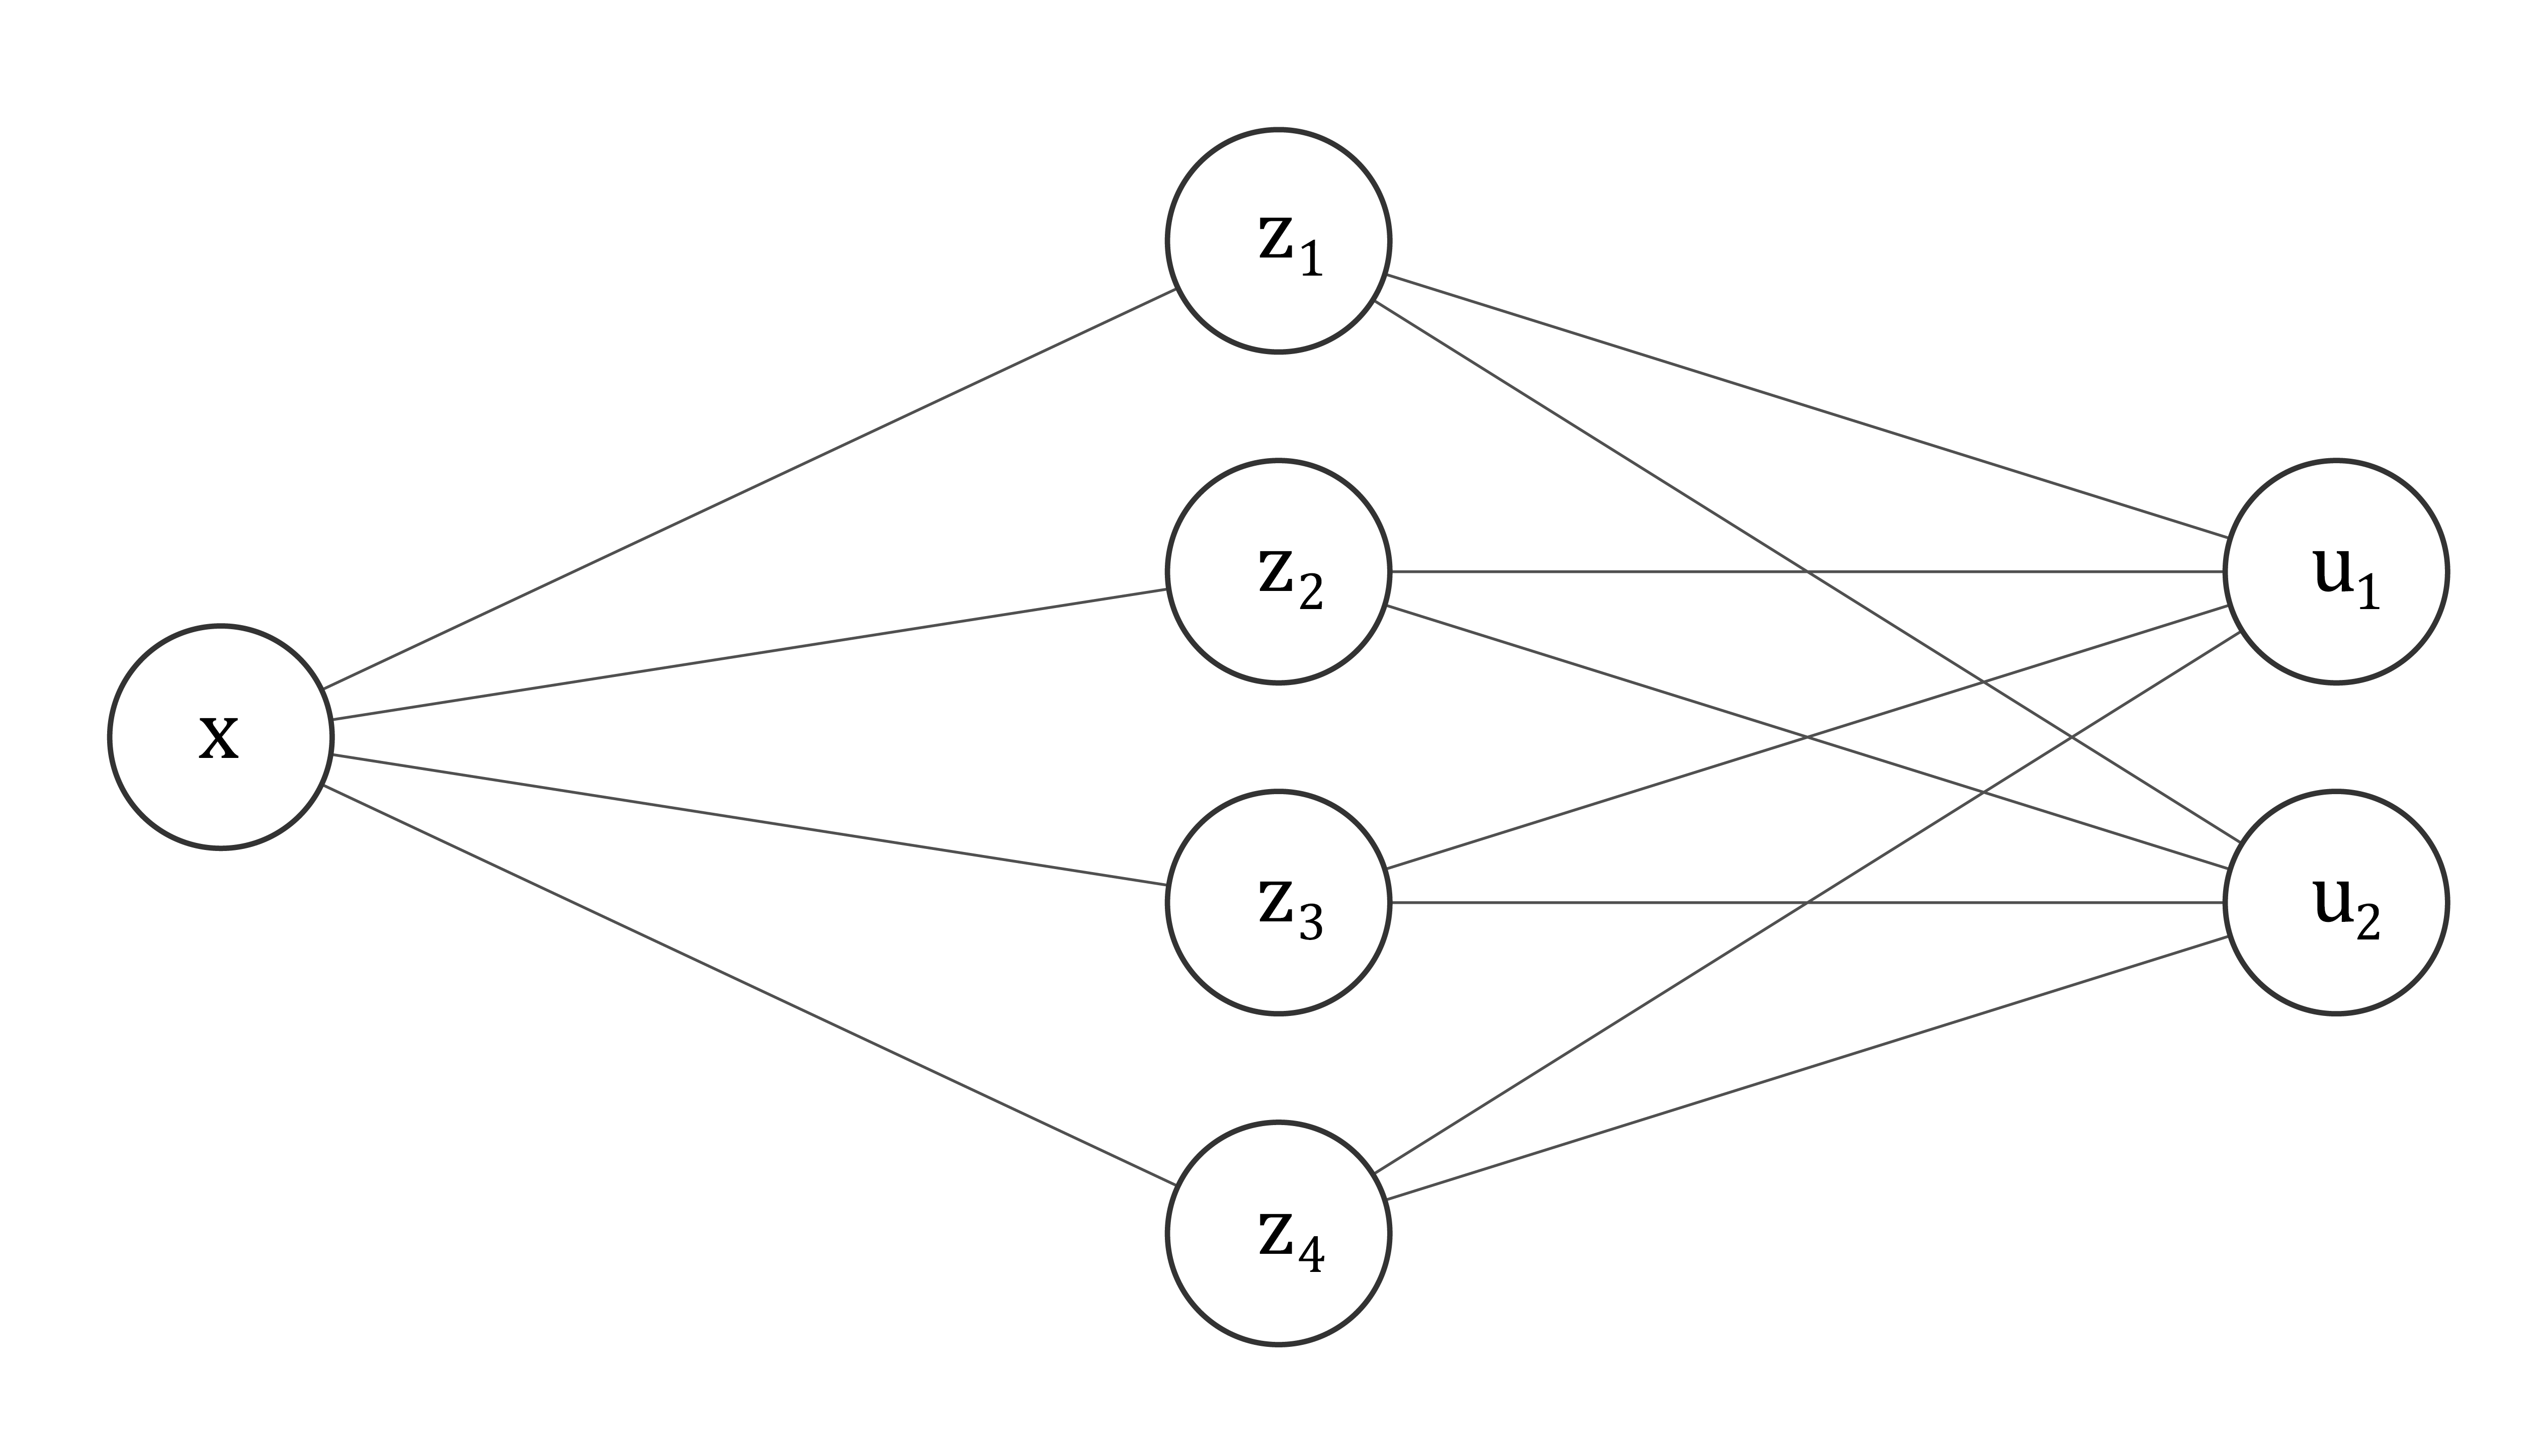
\includegraphics[width=\textwidth]{img/ShallowMLP.png}
        \caption{Shallow multilayer perceptron with $N=3$.}
    \end{subfigure}
\end{figure}

\subsubsection{Basis representation}\label{sec:vpinnsbasis}
** Elaborate on the linear combination of the basis at the last layer, show shallow network formulation with ReLU **

\subsubsection{Variational formulation for VPINNs}\label{sec:vpinnsformulation}
Let $V_K = span(v_1, v_2, \cdots, v_K)$ be the space of the test functions. The helmholtz impedance problem in the context
of VPINNs is defined as finding $u_{NN} \in NN$ such that the loss function
\begin{equation}
    \label{eq:lossfunction}
    \mathcal{L}^2(u_{NN}) = \frac{1}{K} \sum_{k=1}^{K}{|R_k^{(2)} - F_k|^2}
\end{equation}
is minimized. where
\begin{equation}
    \label{eq:vpinnrhs}
    R_k^{(2)} = \int_{a}^{b}{u'_{NN}v'_k} - k^2 \int_{a}^{b}{u_{NN}v_k} - (g_a + \imath ku_{NN}(a))v_k(a) - (g_b + \imath ku_{NN}(b))v_k(b),
\end{equation}
\begin{equation}
    \label{eq:vpinnlhs}
    F_k = \int_{a}^{b}{fv_k}.
\end{equation}
** Explain the local and global quadrature points **\\
** Mention quadrature methods **\\
** Mention redundent weights -> set to 1 -> Liu paper **\\
** Mention initialization of the biases -> uniform -> Liu paper **\\


\section{Results}\label{sec:results}
The results of each method are presented in this section. We define the error of the solution as the $H^1_{(\Omega)}$
norm of difference between the analytical solution $u(x)$, and the solution of the numerical scheme $u_N(x)$ as
\begin{equation}
    \label{eq:H1error}
    ||u(x) - u_N(x)||_{H^1_{(\Omega)}} = ||u(x) - u_N(x)||_{L^2_{(\Omega)}} + ||u'(x) - u'_N(x)||_{L^2_{(\Omega)}},
\end{equation}
where
\begin{equation}
    \label{eq:L2error}
    ||f(x)||_{L^2_{(\Omega)}} = \begin{pmatrix} \int_{\Omega}{|f(x)|^2dx} \end{pmatrix}^{1/2},
\end{equation}
and use this error as a measure to evaluate the solution from each numerical scheme.

\subsection{Finite elements scheme}\label{sec:femresults}
Using the framework described in \autoref{sec:femframework}, we investigated the results of the finite element scheme
for the Helmholtz impedance problem with different frequencies. The results for a relatively moderate $k$  validated
against exact solution are presented in Figures \ref{fig:femMidfreqN050} and \ref{fig:femMidfreqN100}. These plots show how using a finer mesh (bigger $N$)
on the domain improves the quality of the solution. The same trend has been observed for other $k$'s.

\begin{figure}[h]
    \label{fig:femMidfreqN050}
    \centering
    \begin{subfigure}[b]{0.9\textwidth}
        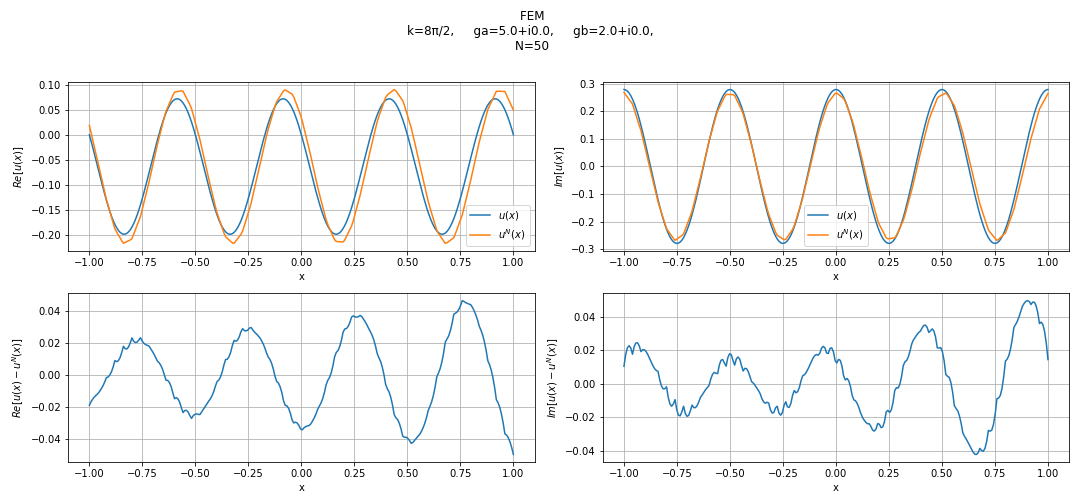
\includegraphics[width=\textwidth]{img/FEM-Const-MidFreq-N0050-sol.png}
        \caption{$u_N(x)$}
    \end{subfigure}
    \vfill
    \begin{subfigure}[b]{0.9\textwidth}
        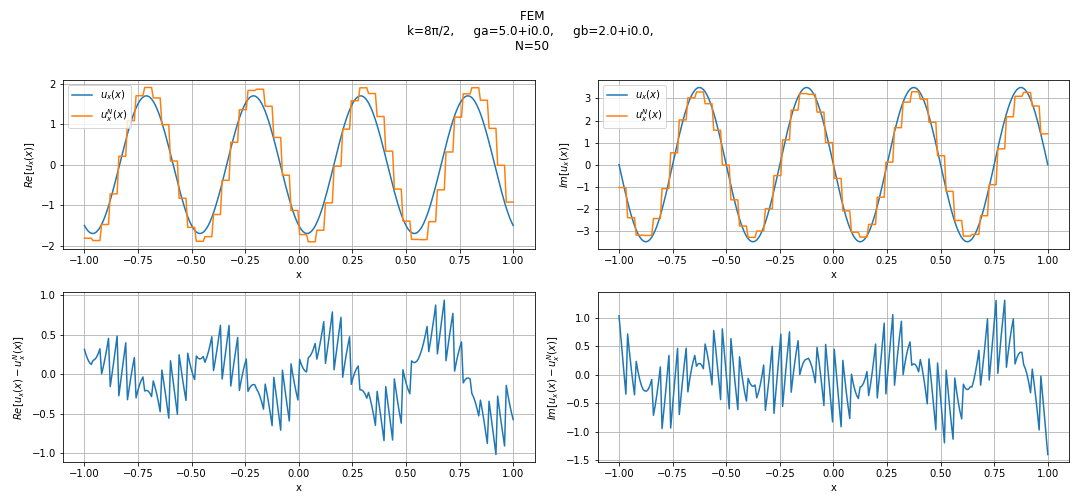
\includegraphics[width=\textwidth]{img/FEM-Const-MidFreq-N0050-der.png}
        \caption{$u'_N(x)$}
    \end{subfigure}
    \caption{$u_N(x)$ (a) and $u'_N(x)$ (b) plotted against the exact solution for a relatively moderate $k$.
    On each subfigure, the bottom row represents the difference between the numerical and exact solutions. The source
    function has a constant value of $f(x)=10$, and other parameters are indicated on the figures.}
\end{figure}
\begin{figure}[h]
    \label{fig:femMidfreqN100}
    \centering
    \begin{subfigure}[b]{0.9\textwidth}
        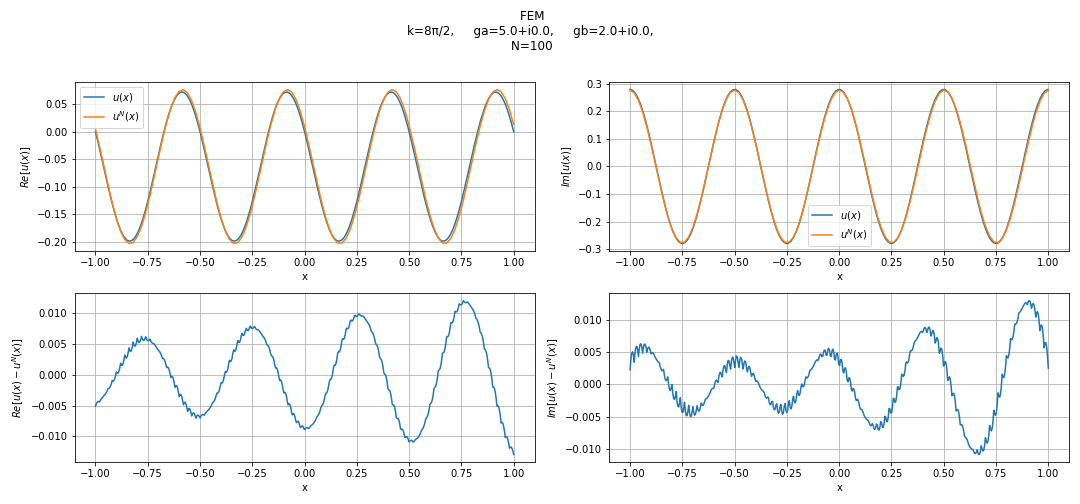
\includegraphics[width=\textwidth]{img/FEM-Const-MidFreq-N0100-sol.png}
        \caption{$u_N(x)$}
    \end{subfigure}
    \vfill
    \begin{subfigure}[b]{0.9\textwidth}
        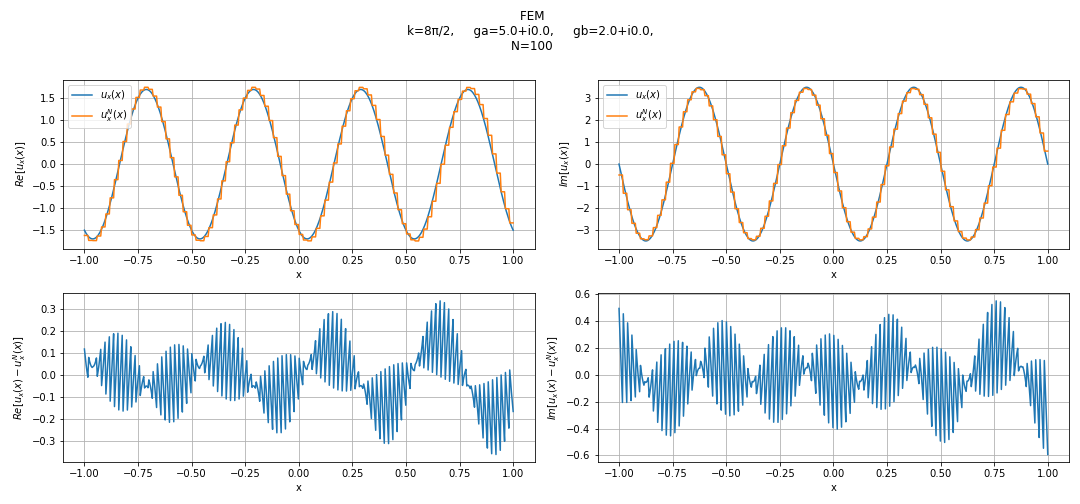
\includegraphics[width=\textwidth]{img/FEM-Const-MidFreq-N0100-der.png}
        \caption{$u'_N(x)$}
    \end{subfigure}
    \caption{$u_N(x)$ (a) and $u'_N(x)$ (b) plotted against the exact solution for a relatively moderate $k$.
    On each subfigure, the bottom row represents the difference between the numerical and exact solutions. The source
    function has a constant value of $f(x)=10$, and other parameters are indicated on the figures.}
\end{figure}

However, for the value of $k$ gets larger, we would have a problem with this method. From the nature of the equation we
know that for larger $k$'s, we have more oscillations in the solution. Since the FEM is estimating the solution with
piecewise linear basis functions in a uniform mesh, the resulting numerical solution will also be piecewise linear. This
will require a minimum number of grid points on each oscillation for the estimation to have a decent accuracy. Consider
the solution in \autoref{fig:femMidfreqN100} where we used 100 grid points. If we wanted to estimate this function with
8 grid points, for instance, it was not possible to even capture the general shape of the function.
This phenomenon is the major observation in \autoref{fig:femorder}, where the H1-error of the numerical solution is plotted against
mesh refinement, $N$, for different values of $k$. For each constant $k$, there is no improvement in the error as we
refine the mesh until a certain $N$, which is called $N_c$ in the rest of the report. However, for $N > N_c$, we can
see the first order accuracy of the method as we expected.
Another important observation is that the value of $N_c$ increases with increasing $k$, which means that for high values
of $k$, the improvement in the accuracy only begins at a very high $N$.
\begin{figure}[h]
    \label{fig:femorder}
    \centering
    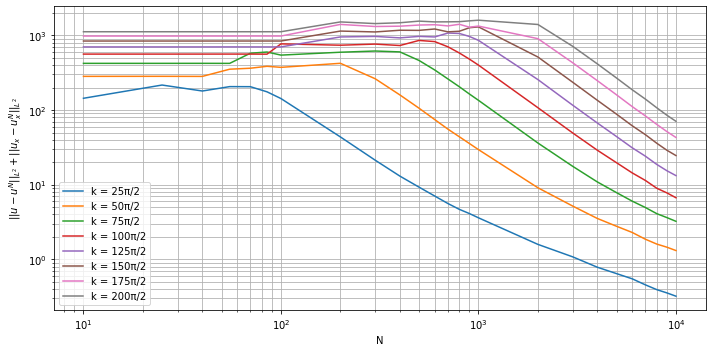
\includegraphics[width=.9\textwidth]{img/FEM-Order-Homog-H1.png}
    \caption{Order of accuracy of the FEM scheme for different values of $k$.}
\end{figure}

\subsection{VPINNs scheme}\label{sec:vpinnsresults}
** empty **

\section{Discussion}\label{sec:discussion}
** empty **

\section{Conclusion}\label{sec:conclusion}
** Suggestions for future work **\\
** Add something innovative **\\
